\chapter{Ford-Fulkerson pathological example}

\section{Intuizione}

Sia $r$ tale che $r^2 = 1-r$:
\begin{itemize}
	\item le capacità iniziali sono $\{1, r\}$
	\item dopo qualche augmentation, le capacità residuali
	      diventano $\{1,r,r^2\}$ (dove $r^2$ = $1-r$)
	\item dopo altre diventano $\{1,r,r^2, r^3\}$
	      (dove $r^3$ = $r-r^2$)
	\item dopo altreancora, diventano $\{1,r,r^2, r^3, r^4\}$
	      (dove $r^4$ = $r^2-r^3$)
\end{itemize}
$$
	r = \frac{\sqrt{5}-1}{2} \rightarrow r^2 = 1 - r
$$

\begin{figure}[H]
	\centering
	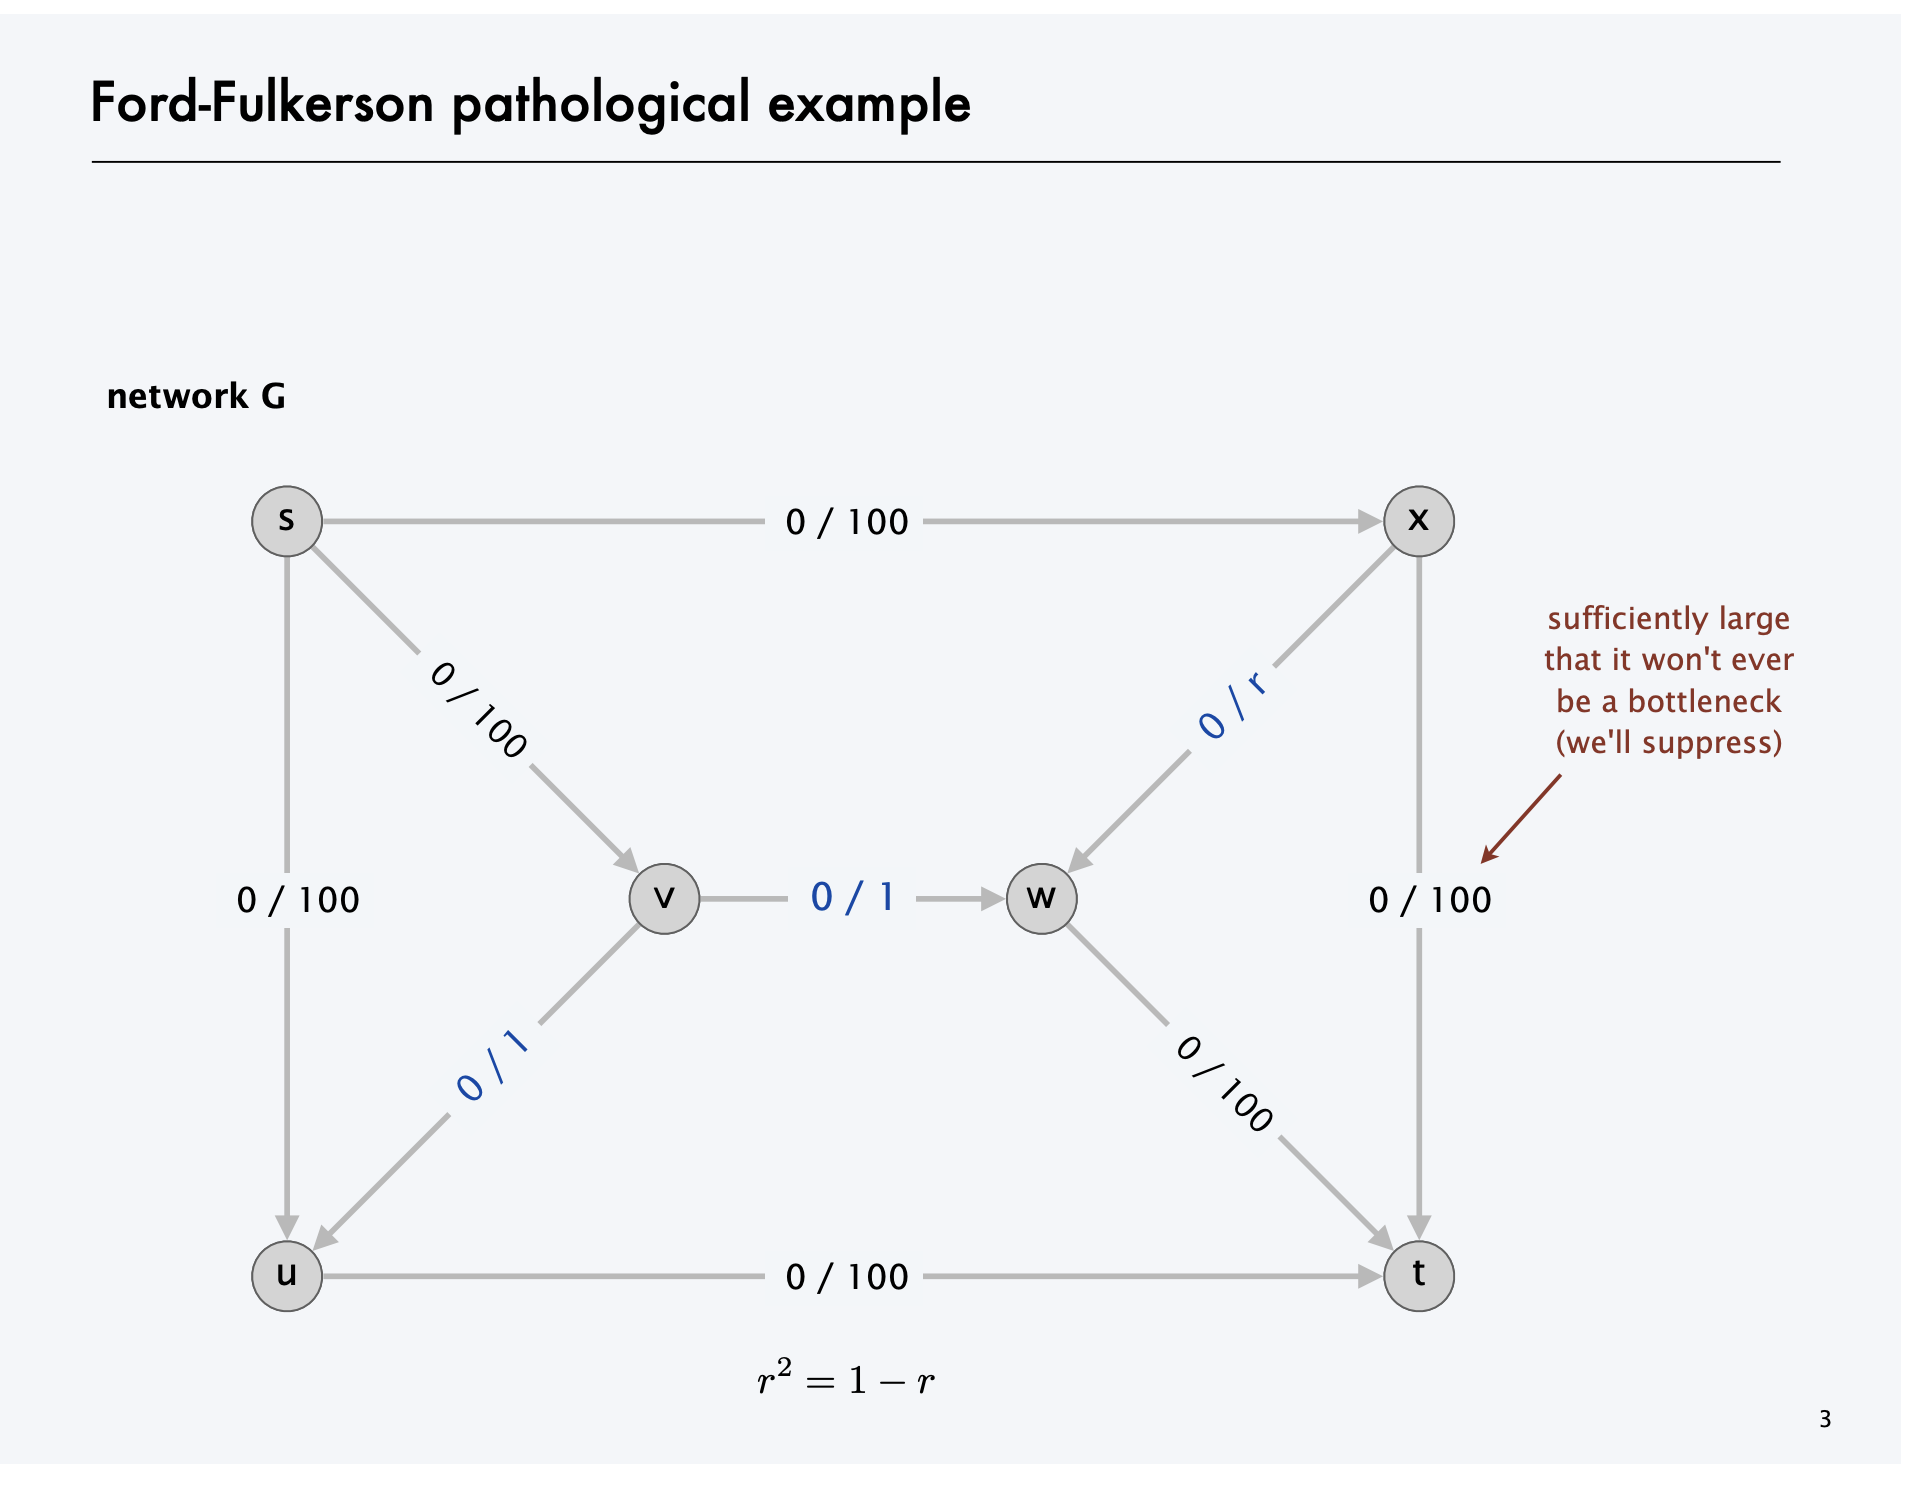
\includegraphics[width=10cm]{capitoli/network_flow/imgs/pathological_example.png}
\end{figure}

Augmenting path 1: $s \to v \to w \to t$. Bottleneck capacity = 1
(v,w).\\

Continuo ad aumentare path che passano per $(v,w)$ e per $(w,v)$ alternati,
quindi aggiungo e tolgo la bottleneck ogni volta. La bottleneck
diminuisce sempre ma va da r a $r^2$ a $r^3$ e cosí via, cosí
l'algoritmo non termina mai:
\begin{itemize}
	\item dopo augmenting path 1: $\{ 1 - r^0, 1, r - r^1 \}$ (flow = $1$)
	\item dopo dopo augmenting path 5: $\{ 1 - r^2, 1, r - r^3 \}$ (flow = $1 + 2r + 2r^2$)
	\item dopo augmenting path 9: $\{ 1 - r^4, 1, r - r^5 \}$ (flow = $1 + 2r + 2r^2 + 2r^3 + 2r^4$)\\
\end{itemize}
\begin{figure}[H]
	\begin{subfigure}{\textwidth}
		\centering
		\begin{subfigure}{.33\textwidth}
			\centering
			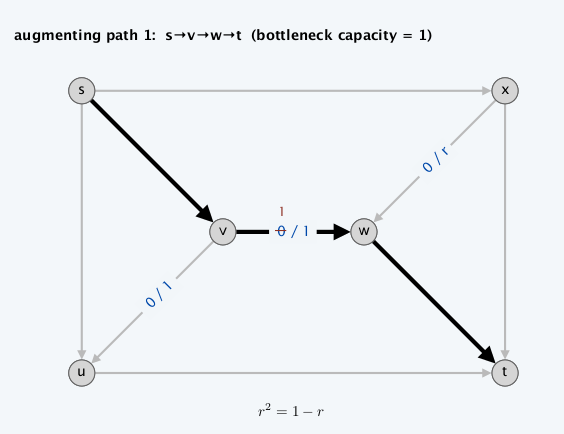
\includegraphics[width=\linewidth]{capitoli/network_flow/imgs/ex1.png}
		\end{subfigure}%
		\begin{subfigure}{.33\textwidth}
			\centering
			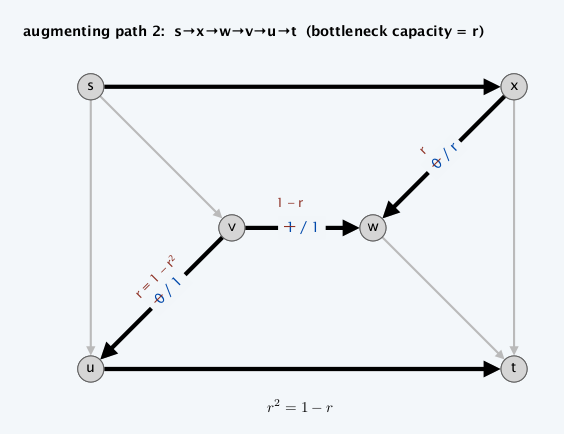
\includegraphics[width=\linewidth]{capitoli/network_flow/imgs/ex2.png}
		\end{subfigure}%
		\begin{subfigure}{.33\textwidth}
			\centering
			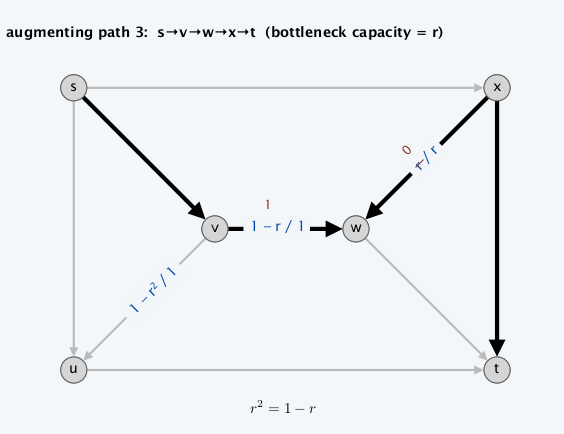
\includegraphics[width=\linewidth]{capitoli/network_flow/imgs/ex3.png}
		\end{subfigure}%
	\end{subfigure}
	\begin{subfigure}{\textwidth}
		\centering
		\begin{subfigure}{.33\textwidth}
			\centering
			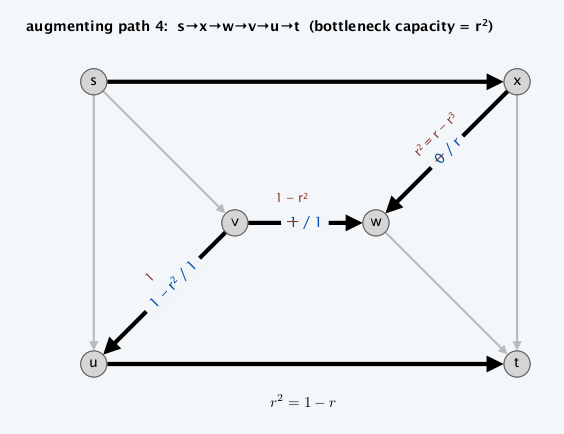
\includegraphics[width=\linewidth]{capitoli/network_flow/imgs/ex4.png}
		\end{subfigure}%
		\begin{subfigure}{.33\textwidth}
			\centering
			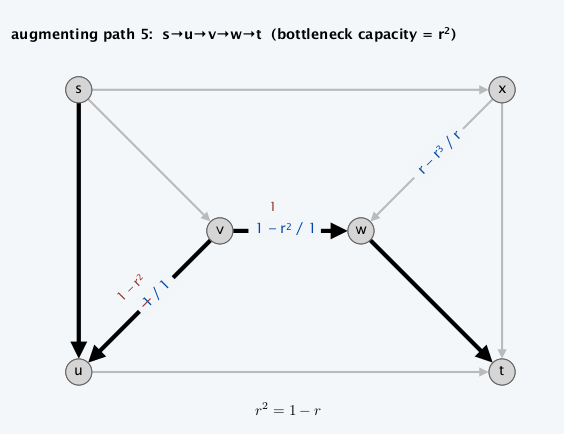
\includegraphics[width=\linewidth]{capitoli/network_flow/imgs/ex5.png}
		\end{subfigure}%
		\begin{subfigure}{.33\textwidth}
			\centering
			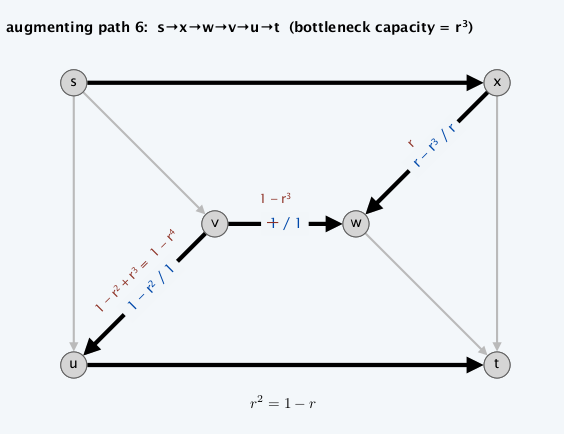
\includegraphics[width=\linewidth]{capitoli/network_flow/imgs/ex6.png}
		\end{subfigure}%
	\end{subfigure}
	\begin{subfigure}{\textwidth}
		\centering
		\begin{subfigure}{.33\textwidth}
			\centering
			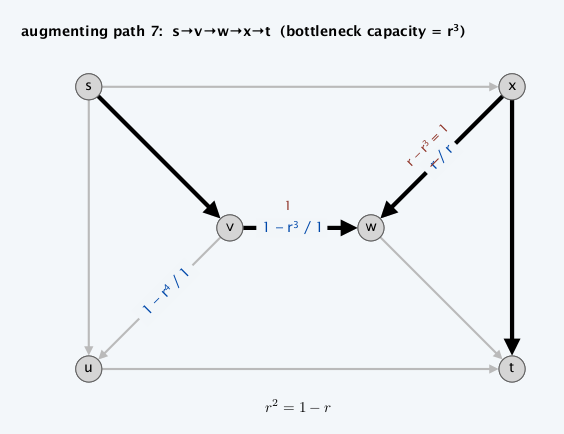
\includegraphics[width=\linewidth]{capitoli/network_flow/imgs/ex7.png}
		\end{subfigure}%
		\begin{subfigure}{.33\textwidth}
			\centering
			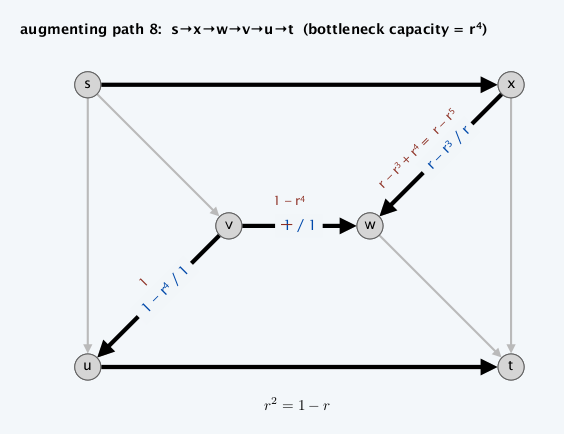
\includegraphics[width=\linewidth]{capitoli/network_flow/imgs/ex8.png}
		\end{subfigure}%
		\begin{subfigure}{.33\textwidth}
			\centering
			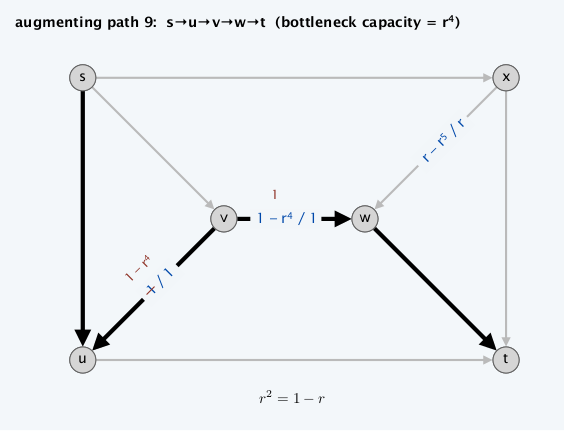
\includegraphics[width=\linewidth]{capitoli/network_flow/imgs/ex9.png}
		\end{subfigure}
	\end{subfigure}
\end{figure}

\begin{myblockquote}
	\begin{minipage}{\textwidth}
		\begin{theorem}
			L'algoritmo di Ford-Fulkerson
			può non terminare e può convergere ad un valore che non è il flusso
			massimo.
		\end{theorem}
	\end{minipage}
\end{myblockquote}

\begin{proof}
	Utilizzando la data sequenza di augmenting
	paths, dopo $(1+4k)^{th}$ di questi path, il valore del flusso è
	uguale a

	$$
		1 + 2 \sum^{2k}_{i=1}r^i \le 1 + 2 \sum^{\infty}_{i=1}r^i = 3 + 2r < 5
	$$

	($r = \frac{\sqrt{5}-1}{2}$) Valore del flusso massimo = 200 + 1.
\end{proof}